% Currently this document is written in English
% !TeX encoding = UTF-8
% !TeX spellcheck = en_US

%Ensure that all odl school LaTeX habits are remarked
\RequirePackage[l2tabu, orthodox]{nag}

%German: remove "english"
\documentclass[english,utf8,biblatex,hyperref]{lni-tex/lni}
% Nice tables using \toprule, \midrule, \bottomrule
\usepackage{booktabs}
% subfigures and subcaptions
\usepackage{subcaption}

%% Begin: Drawings
% use standalone and tikz for high-fid. drawings

% standalone package and config
\usepackage{standalone} % For pre-compiled pictures
\standaloneconfig{mode=buildnew} % only build image if source file is newer

% tikz package and config
\usepackage{tikz} % For Tikz pictures
\usetikzlibrary{
  positioning,
  fit,
  arrows,
  calc,
  backgrounds
}
\usepackage{pgf-umlsd} % UML sequence diagrams
\usepackage[simplified,school]{pgf-umlcd} % UML class diagrams
% UML class diagram overrides
\renewcommand{\umldrawcolor}{black}
\renewcommand{\umlfillcolor}{white}
\tikzstyle{package}=[font=\bf]
% UML class diagram dactor env
\newenvironment{dactor}[1]{
  \def\umlcdDactorName{#1}
  \def\umlcdPackageFit{}
}{
  \begin{pgfonlayer}{background}
    \node[umlcd style, draw, inner sep=0.5cm, fit=\umlcdPackageFit] (\umlcdDactorName) {};
    \node[umlcd style, draw, outer ysep=-0.5, anchor=south west] (\umlcdDactorName caption) at
    (\umlcdDactorName.north west) {\bf\umlcdDactorName : Dactor};
  \end{pgfonlayer}
}
% pgfplots
\usepackage{pgfplots}
%% End: Drawings

%% Begin: Biblatex

%for easy quotations: \enquote{text}, also required by biblatex
\usepackage{csquotes}
% biblatex is included with LNI-class option: `biblatex`, only set bibliography-file:
\bibliography{paper}

% Enable hyperlinked authors when using \citeauthor
% Source: http://tex.stackexchange.com/a/75916/9075
\DeclareCiteCommand{\citeauthor}
  {\boolfalse{citetracker}%
   \boolfalse{pagetracker}%
   \usebibmacro{prenote}}
  {\ifciteindex
     {\indexnames{labelname}}
     {}%
   \printtext[bibhyperref]{\printnames{labelname}}}
  {\multicitedelim}
  {\usebibmacro{postnote}}

% Clear fields we do not need
\iffalse
\AtEveryBibitem{%
  \ifentrytype{article}{%
  }{%
    \clearfield{doi}%
    \clearfield{issn}%
    \clearfield{url}%
    \clearfield{urldate}%
  }%
  \ifentrytype{inproceedings}{%
  }{%
    \clearfield{doi}%
    \clearfield{issn}%
    \clearfield{url}%
    \clearfield{urldate}%
  }%
}
\fi
%% End: Biblatex

%% Begin: lstlistings

% Scala highlighting
\lstdefinelanguage{scala}{
  morekeywords={%
    abstract,case,catch,class,def,do,else,extends,
    false,final,finally,for,forSome,if,implicit,import,lazy,
    match,new,null,object,override,package,private,protected,
    return,sealed,super,this,throw,trait,true,try,type,
    val,var,while,with,yield},
  otherkeywords={=>,<-,<\%,<:,>:,\#,@},
  sensitive=true,
  morecomment=[l]{//},
  morecomment=[n]{/*}{*/},
  morestring=[b]",
  morestring=[b]',
  morestring=[b]"""
}[keywords,comments,strings]

% configuration of lstlisting
\lstset{%
	xleftmargin=0.5cm, % expected by LNI
    captionpos=b,      % expected by LNI
    fontadjust=true,
    columns=[c]fixed,
    keepspaces=true,
    tabsize=2,
    basicstyle=\renewcommand{\baselinestretch}{0.95}\ttfamily,
    commentstyle=\itshape,
    keywordstyle=\bfseries,
    mathescape=true,
    escapechar=§,
}

% macro for inline code
\newcommand{\code}[1]{\lstinline[flexiblecolumns=true,basicstyle=\renewcommand{\baselinestretch}{0.95}\ttfamily]{#1}}

%% End: lstlistings

%% Begin: Acronyms
\usepackage[acronym]{glossaries}
\glsdisablehyper

% define acronyms here:
\newacronym{jvm}{JVM}{Java Virtual Machine}
\newacronym{rdbms}{RDBMS}{relational database management system}
\newacronym{orm}{ORM}{object-relational mapping}
\newacronym{oop}{OOP}{Object-oriented Programming}

% define special names here (we do not create a glossary, so no descriptions are required)
\newglossaryentry{dactor}{name={Dactor},plural={Dactors},description={}}
\newglossaryentry{functor}{name={Functor},plural={Functors},description={}}
\newglossaryentry{relation}{name={relation},plural={relations},description={}}
%% End: Acronyms


%% Begin: Macros
\newcommand{\reactdb}[1]{\textsc{ReactDB}}
%% End: Macros


%% correct bad hyphenation here
\hyphenation{net-works semi-conduc-tor}


% Start of page count 
% ----------------------- filled out by publisher/editor
\startpage{1}
\editor{Vorname Nachname et al.}
\booktitle{Konferenztitel}
% -----------------------

\author[Frederic Schneider \and Sebastian Schmidl]{%
Frederic Schneider \and
Sebastian Schmidl\footnote{Hasso-Plattner-Institut, University of Potsdam, Prof.-Dr.-Helmert-Str. 2-3, 14482 Potsdam, \email{{frederic.schneider,sebastian.schmidl}@student.hpi.de}}
}
\title[An Actor Database System for Akka]{An Actor Database System for Akka}

\begin{document}
\maketitle

% Set to number of authors!
% Authors use each one footnote counter, set this to align the remaining ones.
% E.g. 2 authors --> set to 2, next footnote will be 3
\setcounter{footnote}{2}

\begin{abstract}
Abstract goes here
\end{abstract}

\begin{keywords}
Actor Database System \and Akka \and Scala
\end{keywords}

% Contents
% --------
% !TeX root = paper.tex
% !TeX encoding = UTF-8
% !TeX spellcheck = en_US

% Outline of this paper
        
% !TeX root = ../paper.tex
% !TeX encoding = UTF-8
% !TeX spellcheck = en_US

\section{Introduction}\label{sec:intro}

  % \subsection{Motivation}
  % Impedance mismatch between data and application logic tier
  %  ORM’s try to solve this problem
  % Database scalability

  % motivational statement about importance of parallelization for data processing [sources]
  % "die wichtigsten Motivationspunkte könnt ihr ja aus dem survey ziehen: Objekt mapping explizit machen, skalierbarkeit, fehlertolleranz, wartbarkeit des codes etc. und alles insbesondere wenn es mit stored procedures los geht; die sind der ganz große feind ;-)"
  % data processing close to data storage [sources]
  
  % \subsection{Our Concept}
  % summarize chapters \ref{sec:dactors} and \ref{sec:actor_database_systems} in 2-3 sentences ("auch ein paar sätze mehr")

  % \subsection{Contribution}
  % can we propose our framework? - No "was, bei dem ihr innovativ was neues als erste gemacht ahbt"
  % "Übertragung der Idee von Actor Databases auf das Akka Framework"

  % QUESTION TO TORSTEN: de-facto this is disputable as our framework is more of a application dev framework, so arguably we push data tier into app tier
  % "stellt den vergleich am besten mit einem OR-Mapper wie hybernate her oder JPA. Auch mit einer Datenbank nutzt man i.d.R. frameworks, die den Datenverkehr und das Übersetzen der Business-Objekte in Datenbank-Objekte regeln und somit den Entwicklungsprocess wie ein framework beeinflussen. Man bindet euch wie jede andere bibliothek in ein Programm ein und da dürft ihr wie all diese anderen bibliotheken gerne von frameworks sprechen. der große unterschied ist, dass ihr ganz direkt und nah an den Daten seid und so dinge machen könnt, die andernfalls stored procedures oder andere tiefe Eingriffe aus dem Anwendungscode in die separate Datenbank erfordern. Plus das ganze Datenmanagement ist automatisch verteil-, parallelisier- und skalierbar."

  % \subsection{Paper Overview}
  % summarize and reference all following chapters

  Most web-based applications process data at ever growing rates.
  Whether user logins, the processing and storage of sensor data, or dynamic information provisioning, data is at the center of online applications.
  Multi-core hardware architectures and cluster or cloud deployments allow scaling application logic in terms of computational power.
  Data management systems, however, are at risk of becoming the bottleneck in scaling data-centric software systems.
  Such applications create an increasing demand for scalable data storage solutions, that are capable of fulfilling real-time requirements for OLTP workloads at low latency. % too long, use system instead of 'applications', maybe lose the OLTP

  Traditionally, systems' architectures for these types of software is comprised in two tiers:
  An application logic tier containing the bulk of the system's business logic, as well as a data tier, e.g. a database, which holds the applications data.
  The separation of concerns within this design in terms of concrete functionality depends on the choice of data storage solution.
  A \gls{rdbms} enables data manipulation and the execution of most data-related computation in the data tier, by using e.g. stored procedures and a complex query language.
  However, the monolithic design of conventional \glspl{rdbms} proves a hurdle for scalability and reduces modularity, which has a negative impact on code maintainability. % todo source (maybe from manifesto/reactors)$
  More recently key-value storage solutions have gained popularity especially for high-scale online applications.
  This is due to the fact that their less rigid schema guarantees allow for improved scalability. % source
  The tradeoff of this solution is having to offload much of the data-handling logic into the application tier, thereby increasing load on the application as well as not keeping true to the separation of concerns.

  In either case, the data and application logic tier do not necessarily share a format for data objects.
  Application logic and database exhibit differences in available data types and modelling capabilities.
  Object-oriented programming languages provide concepts such as inheritance and polymorphism, nested objects, and enforce strict object encapsulation.
  \glspl{rdbms} are not able express all of the same concepts due to the representation of data as relations in tables. % maybe it is necessary to elaborate on this
  While data storage solutions with a less rigid schema, such as document-oriented databases, are able to represent, e.g., nested objects, they still face the same problems as \glspl{rdbms} with regard to data formats, inheritance, and encapsulation.
  The described set of difficulties when persisting application state and data objects in a database is commonly referred to as \textit{object-relational impedance mismatch}.
  The use of \gls{orm} tools, such as Hibernate for Java or Active Record for Ruby on Rails, is one approach to provide a middle tier for mapping between the data formats of the application and data tier.
  % However, shortcoming of this approach

  \citeauthor{manifesto} call for a new paradigm for designing a scalable data storage solution using the Actor model \cite{manifesto}.
  The core primitive in this model are actors, which are objects comprised of state and behaviour that execute computational tasks concurrently.
  Individual actors communicate with each other exclusively via asynchronous message passing.
  Incoming messages are stored in a mailbox allowing for the separate and independent processing of each message.
  When receiving a message an actor can modify its state, send a finite amount of messages to other actors, and create new actors.
  An actor's internal state is only available to said actor which encourages a shared-nothing system architecture.
  The self-contained nature of actors and the fact that, through asynchronous message passing, actors provide a lock-free concurrency model, allows for naturally scaling out applications and systems~\cite{vernon2015reactive}.
  % \enquote{The actor model brings OOP back to the system level with actors appearing to developers very much like the familiar model of interacting objects}~\cite{bernstein:orleans}.
  \citeauthor{manifesto} propose an implementation of the data tier using the actor model as a logically distributed runtime using the actor model.
  They predict that this programming abstraction will allow for a modular, scalable application design.

  We build on this idea and present an application development framework for actor-based data-centric application development.
  In this framework actors employ relational structures internally to manage application state and data,
  and provide functionality based on this data in the form of actor behaviour.
  Since these actors are not part of a dedicated database runtime, but are defined and instantiated using the application framework, this approach dissipates the strict line between data and application tier.
  It allows for utilizing and interacting with data objects in the same representation throughout business logic and data storage.

  To our knowledge, we present the first partial implementation of this concept using the Akka framework.
  Comparable, existing work has been presented using the virtual actor concept provided by the Orleans framework for Microsoft .NET.
  Therefor we discuss the differences of the two concepts, such as the need for explicit actor creation, and manual actor lifecycle management in section \ref{sec:related_work}.
  In this section, we also give an outline of the history of Actor model implementations as well as the characteristics of \textit{Actor Database Systems} as proposed by \citeauthor{manifesto}.
  In section \ref{sec:concept} we outline our approach conceptually in more detail,
  before explicitly describing the implementation of our proof-of-concept framework, as well as some examples for usage patterns in section \ref{sec:framework}.
  We present setup and evaluation of experiments on the memory overhead introduced by the use of actors for data storage using our framework in section \ref{sec:experiments},
  and offer a concluding statement about this and future work in \ref{sec:conclusion}.
  


% !TeX root = ../paper.tex
% !TeX encoding = UTF-8
% !TeX spellcheck = en_US

\section{Related Work}\label{sec:related_work}

  The Actor model, as described in the previous section, denotes a mathematical concept for concurrent computation which dates back to the early 1970's.
  It has gained popularity and been implemented anew as language extensions or frameworks for existing object-oriented and functional languages, such as C\#, Java, and Scala, in the mid-2000's.
  In this sections we give an outline of the recent history of Actor model implementations,
  discuss differences of the conventional actor model and the virtual actor model used in the Orleans framework,
  and elaborate on the notion of \textit{Actor Database Systems} and their requirements.

  \subsection{Actor Model}
  % https://www.brianstorti.com/the-actor-model/
  % https://en.wikipedia.org/wiki/Actor_model
  % https://doc.akka.io/docs/akka/2.5.3/scala/guide/actors-intro.html
  % https://link.springer.com/content/pdf/10.1007%2F978-3-642-39038-8.pdf#page=318 (page 302)
  Various programming languages and libraries implement the actor model and provide the corresponding functionality:
  The Erlang programming language supports concurrency using the actor programming model and is designed for distributed and highly available systems in the telecommunication sector~\cite{armstrong:erlang}.
  The Scala programming language's standard library included an actor model implementation for concurrent computation starting in 2006, which has now been deprecated for the Akka library~\cite{Haller:2012}.
  Akka implements the actor model for the \gls{jvm} and can be used with the languages Java and Scala~\cite{akka}.
  Akka.Net is a community-driven port of the Akka toolkit for the .NET platform in the languages C\# and F\#~\cite{akka.net}.

  \subsection{Virtual Actor Model}
  While the actor programming model allows for low-level interaction with the actor lifecycle management, handling race conditions, physically distributing actors, and failure handling, the virtual actor programming model raises the abstraction level of actor objects.
  It still adheres to the plain actor model, but treats actors as virtual entities.
  In this model actor lifecycle management and distribution is managed by the framework or runtime and not by the application developer.
  The physical location of the actor is transparent to the application.
  This model is comparable to virtual memory, which allows processes to access a memory address whether it is currently physically available or not.

  The virtual actor model was introduced with the Orleans framework for .NET by Microsoft Research~\cite{bernstein:orleans}.
  In Orleans, actors (virtually) exist at any time.
  There is no possibility to create an actor explicitly.
  Instead, this task is handled by the language runtime, which instantiates actors on demand.
  The runtime's resource management deals with unused actors and reclaims their space automatically.
  The Orleans runtime guarantees that actors are always available.
  This means, that in the view of an application developer an actor can never fail.
  The runtime will deal with crashing actors and servers and recreate missing actor incarnations accordingly.

  The corresponding framework for the \gls{jvm} is Orbit~\cite{orbit}.
  In Orbit, a virtual actor can be active or inactive.
  But those two states are transparent to the application developer.
  Similar to Orleans, messages to an inactive actor in Orbit will activate it, so the actor can receive the sent message.
  Actor state in Orbit is usually stored in a database, which allows for activation and deactivation of actors at runtime.
  During activation of an actor, the state is recovered from persistent database storage.
  Before the actor is deactivated, its state is written back to the database.

  %Discussion about virtual actors in Akka.NET (also applies to Akka): \url{https://github.com/akkadotnet/akka.net/issues/756}
  %-- somewhat implemented with cluster sharding project
  Akka provides similar functionality with Akka Cluster Sharding~\cite{akka:clustersharding}.
  It introduces the separation of virtual and physical Akka actors.
  Actors are first grouped into shards, which can then be located at different physical locations.
  The distribution of the shards and their actors is managed by the framework and it also deals with the routing of the messages and re-balancing the shards to different nodes based on different strategies.
  A developer must not know, where a specific actor is physically located to send messages to it.
  Akka Cluster Sharding also supports passivation of actors.
  This means that unused persistent actors can be unloaded to free up memory (passivation).
  A message to passive actors will instruct the framework to load it back into memory.

  In this paper we denote virtual actors as vactors to clearly distinguish actors of the actor model (actor) from those of the virtual actor model (vactor).

  % Note for possible deletion.


  \subsection{Actor Database Systems}
  The actor and virtual actor programming model is increasingly used to build soft caching layers and cloud applications for various purposes~\cite{erlang_uses,akka_uses,orleans_uses}.
  This shows the appeal of the programming model that allows developers to easily develop modular and scalable software, which can be deployed in the heterogenous parallel cloud computing infrastructure.
  
  Despite its popularity for application development, the actor programming model and actor programming frameworks lack state management capabilities, specifically for data-centric applications.
  The developer has to decide how to handle state persistence and how to satisfy the failure and consistency requirements of the application, because actor model implementations do no provide atomicity or consistency guarantees for state across actors.
  \Citet{manifesto} find a need for state management guarantees in actor systems and propose to integrate actor-based programming models in database management systems.
  The authors postulate that \textit{Actor Database Systems} should be designed as a logical distributed runtime with state management guarantees.
  They should allow for and encourage the design of modular, scalable and cloud-ready applications.
  \Citet{manifesto} outline four tenets that identify an \textit{Actor Database System} and specify needed features in their manifesto:
  \begin{description}
    \item[Tenet 1] Modularity and encapsulation by a logical actor construct
    \item[Tenet 2] Asynchronous, nested function shipping
    \item[Tenet 3] Transaction and declarative querying functionality
    \item[Tenet 4] Security, monitoring, administration and auditability
  \end{description}

  Practical work on actor database systems has been done using the Orleans framework.
  \Citet{Shah:reactdb} tightly follow the propositions of the manifesto and present \reactdb{},
  an in-memory OLTP database system that is programmed via application-defined actors with relational semantics, called reactors.
  A reactor is a logical entity encapsulating state as relations, with
  asynchronous function processing capability, which typically represents a application-level scaling units.
  Within individual reactors classic declarative querying can be used, but across actors explicit asynchronous function calls must be defined.
  \citeauthor{Shah:reactdb} show that transactions across reactors can have serializability guarantees.
  \Citet{Eldeeb:transactions} introduce a new transaction protocol for distributed actors improving the throughput compared to the two-phase commit protocol.
  \Citet{Bernstein:indexing} explore indexing mechanisms in an actor database system.
  They propose a new indexing architecture based on the Orleans framework that is fault-tolerant and eventually-consistent.

  \Citet{biokoda:actordb} takes a different approach to combine actor programming models and relational database systems.
  In their development actorDB, an actor encapsulates a full relational SQL database using the SQLite database engine\footnote{\url{https://www.sqlite.org/about.html}}.
  Actors can be deployed in an distributed cloud environment and communicate asynchronously.
  The database is ACID-conform and enforces consistency across actors with the Raft consensus protocol~\cite{raft}.
  The database can used via the MySQL-protocol.

  Most practical research in the field of actor database systems has been presented in conjunction with the Orleans framework and the Erlang programming language.
  The open-source project \textit{Actorbase} by \citet{actorbase} constitutes a key-value store implementation utilizing Akka actors for horizontal scaling and partitioning.
  In this research database system, partitions are managed by storekeeper actors while inter-partition lookup and indexing is managed by so-called storefinder actors.
  This approach is limited to a key-value store function set and does not provide functionality corresponding to the relational features discussed earlier.


% !TeX root = ../paper.tex
% !TeX encoding = UTF-8
% !TeX spellcheck = en_US

\section{Domain Actor Database Framework}\label{sec:concept}
  Our actor databases system consists of two building blocks: \emph{domain actors} and \emph{\glspl{functor}}. These two concepts allow for the definition of application data within the application itself. Since both are based on actor model principles, they make the database system modular, cloud-ready, and scalable. In this section, we introduce both domain actors and \glspl{functor}.
  
%  Our concept is based on the idea of actor database systems as introduced by \citet{manifesto}.
%  The combination of application and data tier provides considerable advantages for data-centric systems.
%  This architecture allows leveraging domain and application knowledge to dynamically model the data layout, especially concerning data partitioning and replication schemes.
%  This makes the database system modular, cloud-ready, and scalable.
  % add here: why is it better to use domain knowledge to partition and distribute data?

  \subsection{Domain Actors -- Encapsulation of Data}\label{sec:dactors}
    Similar to \citet{Shah:reactdb}, we introduce a special type of actor, called \gls{dactor}, that acts as an application-defined scaling unit.
    \Glspl{dactor} can be used to model application-domain objects and encapsulate the object's state and application logic in an actor.
    Using actors for this enforces technical encapsulation of state access due to the purely private state in actors and the need of explicit asynchronous messaging between the actors.
    The encapsulation also makes it easier to reason about state changes, bugs, and other failures, as only code within the \gls{dactor} can change the corresponding state.

    % internal data management with relations
    In-memory data contained within a \gls{dactor} instance is managed in a data structure called \emph{\gls{relation}}.
    One \gls{dactor} can contain multiple \glspl{relation}.
    A \gls{relation} is, similarly to a table in the relational database model, defined as a multiset of tuples following a predefined schema.
    \Glspl{relation} provide an SQL-like interface to query and manipulate the contained data, so known and proven syntax and semantics can be used to define \gls{dactor}-behavior.
    \Glspl{relation} form a typed, \gls{dactor}-internal data model.
    Using \glspl{dactor} to implement a database leads to a modeling approach that is different to Entity-relationship modeling.
    The following example discusses the conceptual differences between the two in more detail.

    We consider the example of a web application with information on movies similar to the imdb.com or rottentomatoes.com websites.
    A standard query for those websites is to display a film with its description and cast.
    A traditional data layout might be comprised of two entities: \textit{Film} containing the film's ID, title, description and release date and \textit{Actor} containing the actor's ID and name.
    Those two entities might be in a N-to-M relation (\textit{Cast}) with an attribute showing the actor's role in the film.
    In contrast to the relational model, our model, shown in \cref{fig:film_diagram}, consists of one \gls{dactor} type and two \glspl{relation} and is denormalized.
    The information contained in the \textit{Actor} entity is distributed across the \code{Cast} \glspl{relation}.
    This allows us to answer the standard queries from one single actor instance without needing to join the answers from different, possibly physically distributed \gls{dactor} instances.

    This approach to layout an application's data results in much smaller data sizes per \gls{dactor} compared to typical database tables and enables many business-logic-driven approaches to scaling, data partitioning, and caching.
    The trade-off, however, is a large number of \gls{dactor} instances and a (partially) denormalized schema.

    \begin{figure}
      \centering

      \begin{subfigure}[b]{0.44\textwidth}
        \centering
        \includestandalone[width=\textwidth]{pictures/tikz/dactor_diagram}
        \caption{Graphical representation of the \texttt{Film} \gls{dactor} type definition.}
        \label{fig:film_diagram}
      \end{subfigure}\hfill
      \begin{subfigure}[b]{0.54\textwidth}
        \centering
        \scriptsize
\begin{lstlisting}[language=Scala]
class Film(id: DactorId) extends Dactor(id) {
  override protected val relations = {
    Film.Info -> SingleRowRelation(Film.Info),
    Film.Cast -> RowRelation(Film.Cast)
  }
  override def receive: Receive =  //Dactor behavior
}
object Film {
  object FilmInfo extends RelationDef {
    val title = ColumnDef[String]("title")
    val description = ColumnDef[String]("description")
    val release = ColumnDef[ZonedDateTime]("release")
  }
  object Cast extends RelationDef {
    val actorId = ColumnDef[DactorId]("actor_id")
    val name = ColumnDef[String]("actor_name")
    val rolename = ColumnDef[String]("role_name")
  }
}
\end{lstlisting}
        \subcaption{Example code using our framework.}
        \label{lst:film_definition}
      \end{subfigure}
      \caption[\texttt{Film} Dactor type definition with two relations of the example application.]{\code{Film} \gls{dactor} type definition with two relations from the example application.}
      \label{fig:film_dactor_definition}
    \end{figure}

    % logic and processing capabilities
    As \glspl{dactor} not only contain data, but also the corresponding domain logic, computation is executed concurrently.
    Actors provide single-threaded semantics, which makes enforcing constraints on data stored inside one \gls{dactor} easy.
    While state querying and modification within \glspl{dactor} is possible in a declarative way, the application developer can explicitly define the communication across all kinds of actors via asynchronous messages.
    The explicit messaging differentiates \glspl{dactor} from \citet{Shah:reactdb}'s reactors, as reactors can be used as relational entities and hide the message passing from the developer.
    
    To illustrate the definition of a \code{Dactor} in code, we show the definition of \code{Film}'s data model in \cref{lst:film_definition}.
    Developers can model the application's domain objects by defining \gls{dactor} types as subclasses of the framework-provided \code{Dactor} class in a declarative way.
    Instances of such user-defined \gls{dactor} types are managed by the framework and are available for messaging in a consistent namespace.
    Using the column's predefined data types, all functions support compile-time type-safety.
    Due to the \gls{dactor} system sharing the application's runtime and programming environment, these data or object types are equal to the types handled in any application logic.
    Thus, this approach helps eliminate the impedance mismatch between application logic and data tier with regard to handled data types and object (de-)serialization.

  \subsection{Functors -- Encapsulation of Queries}
    \Glspl{dactor} can answer queries via explicit, asynchronous messaging, {i.e.}, they answer a query with their local data.
    Sometimes, however, queries need be answered by several actors.
    In such cases, it makes sense to encapsulate the processing in a new, short-living actor that we call \gls{functor}.
    \Glspl{functor} are the framework's concepts that enable inter-\gls{dactor} communication and computations.
    They communicate with (usually multiple) \glspl{dactor}, track the completion of a query, handle the state of pending requests, and resolve failure cases.
    Every actor can create a new \gls{functor} to encapsulate multiple requests to \glspl{dactor}.
    The \gls{functor} handles the message processing and sends the final result or a failure message back to its creator.
    Since all Akka actors live in hierarchical parent-child relationships, \glspl{functor} are always created by an actor as a child.
    This Akka-specific hierarchical relationship enables notifying the calling actor even in case of unforeseen crashes of the \gls{functor} themselves, which in turn allows to trigger error handling, e.g. retrying the \gls{functor} execution.
%  \subsection{Comunication Patterns for Domain Actors}\label{sec:dactor_comm}
%    Not all computation can be done with the information residing in a single \gls{dactor}.
%    Hence, communication between \glspl{dactor} is required.
%    Explicit, asynchronous message passing allows application developers to chose the right messaging pattern for their use case.
%    The choice is heavily influenced by the data layout used for the \glspl{dactor} and sets the level of parallelization and the network-load for the computation.
    In our actor database system, we consider three messaging patterns for inter-\gls{dactor} communication, which are shown in \cref{fig:comp_patterns}.
    These patterns are provided as messaging primitives by the framework and can be combined to create more complex message flows and computational models:

    \begin{figure}
      \centering
      \begin{subfigure}[t]{0.32\textwidth}
        \centering
        \includestandalone[width=\textwidth]{pictures/tikz/cascading_computation}
        \subcaption{Cascading Computation}
        \label{fig:comp_pattern_1}
      \end{subfigure}\hfill
      \begin{subfigure}[t]{0.32\textwidth}
        \centering
        \includestandalone[width=\textwidth]{pictures/tikz/sequential_computation}
        \subcaption{Sequential Computation}
        \label{fig:comp_pattern_2}
      \end{subfigure}\hfill
      \begin{subfigure}[t]{0.32\textwidth}
        \centering
        \includestandalone[width=\textwidth]{pictures/tikz/concurrent_computation}
        \subcaption{Concurrent Computation}
        \label{fig:comp_pattern_3}
      \end{subfigure}
      \caption{Inter-\gls{dactor} communication patterns. Gray bars indicate that an actor holds state that is related to the showed message flow.}
      \label{fig:comp_patterns}
    \end{figure}

      \textbf{Cascading Computation} is a pattern where a high-level message to an initial \gls{dactor} (\gls{dactor} A) triggers successive messages to other \glspl{dactor}, which are hidden from the original requester.
      Following \glspl{dactor} can also trigger further messages themselves.
      As one can see in \cref{fig:comp_pattern_1}, this pattern is comparable to function calls in Object-oriented Programming.
      But contrary to simple function calls, messages in this pattern are sent asynchronously.
      This means that the requesting \gls{dactor} has to manage the state of pending responses.
      This clutters the domain logic in the \gls{dactor} and leads to complex and error-prone code.
      If used sparsely, this pattern supports separation of concerns and the tell-don't-ask paradigm.

      \textbf{Sequential Computation} is used for queries that consist of consecutive steps, where each step depends on the previous step's result, such as filter chains.
      This pattern can be implemented via the aforementioned \glspl{functor}.
      Using a \gls{functor} to process the consecutive steps of the computational chain relieves \gls{dactor} A from dealing with intermediate state, because it is managed by the \gls{functor}.
      Each \gls{functor} deals with only one request-response pair at a time, which leads to simple state and processing logic for the \gls{functor} itself.

      \textbf{Concurrent Computation} is a another messaging pattern based on \glspl{functor} to encapsulate the processing of multiple request-response pairs.
      The concurrent \gls{functor} sends messages to several \glspl{dactor} in parallel and collects the results when they are finished to forward them to its creator.
      It allows for highly parallelized computations as all involved \glspl{dactor} are messaged at the same time and calculate their responses concurrently.
      
    In summary, explicit message handling in \glspl{dactor} is used to implement the cascading communication pattern; sequential and concurrent \glspl{functor} are the framework's concepts to enable inter-\gls{dactor} communication and computations.
    Returning to the web application example, we now want to add a new film to the database using the \gls{functor} concept.
    This involves changes to a new \code{Film} and the corresponding \code{Studio} \gls{dactor} instances.
    We can combine the concurrent and sequential \glspl{functor} to implement this functionality, which is displayed in \cref{fig:functor_diagram}.
    Both sequential \glspl{functor} are comprised of two subsequent steps:
    They retrieve information from one \gls{dactor} to update the other one.
    They are independent of each other, so they can be executed in parallel, which is done by using the concurrent \gls{functor}.
    It only sends a successful response to its caller after both sequential \glspl{functor} have sent their responses to the concurrent \gls{functor}.
    
    \begin{figure}
      \centering
      \includestandalone[width=\textwidth]{pictures/tikz/functor_diagram}
      \caption{Component diagram indicating the message flow through \gls{functor} objects and their supervision by the calling actor. Arrow and dashed arrow pairs indicate corresponding request and response messages. The outgoing requests of each sequential \gls{functor} are numbered to indicate their order.}
      \label{fig:functor_diagram}
    \end{figure}      
      
    \subsection{System Details}\label{subsec:framework_discussion}
      \emph{Data partitioning} in an actor database system differs fundamentally from common partitioning techniques used in relational databases.
      While large tables are typically partitioned based on a specific column's value or the hash thereof, our framework provides \glspl{dactor} as entities for data encapsulation and partitioning.
      \Glspl{dactor} can be provisioned across multiple virtual runtimes and physical machines, because every \gls{dactor} instance is independent of the others and the only mean of communication is message passing.
      As such, they provide flexible, fine-grained data partitioning based on application needs.
      
      The distributed nature of the database system introduces the new problem of partition or \emph{actor discovery}.
      The framework maintains a unified namespace, in which each \gls{dactor} instance is identified by its \gls{dactor} type and a unique ID.
      In fact, querying a specific \gls{dactor} just requires obtaining the messaging address from the name-service and sending a message to it.
      In case of a multi-node deployment, this is complemented by Akka's Cluster Sharding component, which routes the messages to the right physical host.
      
      Finally, \emph{failure handling}, especially with regard to computations relying on multiple \glspl{dactor}' data, requires careful monitoring due to \gls{dactor} distribution.
      Building on Akka's parent-child supervision concept, our framework allows for transparent failure handling configurations.
      Failures can be handled within \glspl{dactor} if appropriate.
      In case of multi-\gls{dactor} queries a fail-fast approach is chosen to allow calling actors to react to exceptions in a timely manner.

% !TeX root = ../paper.tex
% !TeX encoding = UTF-8
% !TeX spellcheck = en_US

\section{Domain Actor Database Framework}\label{sec:framework}
% Describe implementation details and framework design

After describing the general concept of an \textit{Actor Database System}, we present the implementation of an proof-of-concept application development framework, which allows for the definition of an application's data model and the provisioning of corresponding \glspl{dactor} as part of the application runtime.

The framework provides the aforementioned features for developers:
\begin{itemize}
  \item Declarative data model definition using \glspl{dactor}
  \item SQL-like interface for accessing and manipulating internal data within \glspl{dactor}
  \item \Gls{functor} objects for procedures, which rely on data contained in multiple \glspl{dactor}
\end{itemize}

% Tenets
These features relate to three of the four core tenets that define an \textit{Actor Database System} according to \citeauthor{manifesto}'s manifesto~\cite{manifesto}:
\textbf{Tenet 1} calls for the use of actors to achieve a modular logical model for data encapsulation.
\Gls{dactor} instances are in-memory storekeepers for application data.
They satisfy the actor definition and support high modularity.
Furthermore, \glspl{dactor} provide a model for concurrent computation of predefined functionality that increases locality of data accesses.
This is part of the requirements described in \textbf{Tenet 2}.
All communication between \glspl{dactor} is asynchronous to leverage the advantages of increasingly parallel hardware.
\Glspl{functor} allow for the definition of functionality using multiple actors' data and are executed asynchronously as well.
The possibility to define these \glspl{functor} as well as \gls{dactor} behavior in a declarative way relates to the second part of \textbf{Tenet 3}.
Due to their single-threaded computation model, \glspl{dactor} can be argued to enforce internal consistency by default.
In principle, \glspl{functor} allow for the implementation of further transaction protocols to ensure inter-\gls{dactor} consistency guarantees.
Since the requirements listed under \textbf{Tenet 4} relate mostly to production-ready database products, we do not implement or investigate them in this research project.
The functionality described by \citeauthor{manifesto} in tenets one through three suffices the investigation of the practical feasibility and implications of the actor database concept.

% Tech
Our proof-of-concept framework is developed using the Scala programming language and the Akka framework.
This implementation marks, to the best of our knowledge, the first practical examination of the actor database concept using Akka and the classical actor programming model.
While the Orleans framework, which has been used in earlier related work, provides virtual actors with automatic lifecycle management, Akka allows for and requires direct control over an actor's lifecycle.
% As \glspl{dactor} directly build on the provided Akka actor implementation, these considerations directly apply to them.
These considerations directly apply to \glspl{dactor} as they are built on top of the Akka actor implementation.
% More Discussion of the implication that this allows for more detailed configuration and custom \gls{dactor} idle behavior in Discussion

\subsection{Internal Data Management}

In-memory data that is contained within a \gls{dactor} instance is managed in a data structure called relation.
% Relations contain a multiset of records or tuples which follow a pre-defined schema.
A relation, similarly to a table in the relational database model, is defined as a multiset of tuples following a predefined schema.
This schema is comprised of column definitions whereby every column is defined by a name and a data type.
%They provide a type-safe, SQL-like interface for querying and manipulating contained data.
%The features and interface they provide is inspired by SQL to allow for simple data manipulation using known and proven syntax and semantics when defining a \gls{dactor}'s behavior.
%All manipulation and query functionality on a relation's data provide compile-time type safety based on these column's predefined data types.
Relations provide an SQL-like interface to query and manipulate the contained data, so known and proven syntax and semantics can be used to define \gls{dactor}-behavior.
Using the column's predefined data types, all functions support compile-time type-safety.
Due to the \gls{dactor} system sharing the application's runtime and programming environment, these data or object types are equal to the types handled in any application logic.
Thus, this approach eliminates the impedance mismatch between application logic and data tier with regard to handled data types and object (de-)serialization.

% This could be Usage / Discussion
Due to the similarities between relations and tables known from the relational database model, we want to discuss the conceptual differences between the two.
While relations can be used to model much of the same information as is commonly represented using tables, the \textit{Actor Database System} and specifically the concept and framework we present relies on \glspl{dactor} as models for application domain objects.

For clarification consider the following example of a web application with information on films and (human) actors similar to the imdb.com or rottentomatoes.com websites.
A traditional data layout might be comprised of two tables containing information on films and actors, respectively.
Using \glspl{dactor} to represent discrete domain-level objects, a single \gls{dactor} of the type film represents a single, specific film and encapsulates all corresponding data.
This approach to layout an application's data results in much smaller relation sizes than typical table sizes and enables many business-logic-driven approaches to scaling, data partitioning, and caching, which are discussed in section~\ref{subsec:discussion}.

\subsection{Domain Actor Design}\label{subsec:domain_actor_design}

Developers can model the application's domain objects via extending the framework's abstract \code{Dactor} class.
Instances of such user-defined \code{Dactor} types are managed by the framework and are available for messaging in a consistent namespace.
A \code{Dactor} type definition is comprised of the types internal data schema, i.e. relations, and its functionality to process said data.
Note that, since \glspl{dactor} can logically encapsulate multiple data sets and state information, they can and often do comprise multiple relations.

To illustrate the definition of \code{Dactor}s we use the formerly introduced example.
The application in its simplest form consists of two \code{Dactor} types modeling the domain entities: \code{Film} and \code{Actor}.

\code{Film} \gls{dactor} instances store information about a specific film, such as its title, release date, a description, and a unique id, but also information about its starring actors:
The actor's (person) name, the name of the role they portray, as well as the corresponding \gls{dactor} instance id.
The \code{Actor} instances comprise additional information on the person, such as the date of birth, but also a list of films they starred in, including the name of the role they portray, the film's title, and the id to the \code{Film} \gls{dactor}.
The definition of the \code{Film}'s data model is shown in listing~\ref{lst:film_definition}.

\begin{lstlisting}[caption=Film Dactor type definition using the actordb framework, label=lst:film_definition, language=Scala]
object Film {
  // Definitions of relations contained in Film type Dactors
  object Info extends RelationDef {
    // column with name "title" and data-type String:
    val title = ColumnDef[String]("title")
    val description = ColumnDef[String]("description")
    // rich datetime data-type column:
    val release = ColumnDef[ZonedDateTime]("release")
  }

  object Cast extends RelationDef {
    // foreign key relating to an Actor type Dactor instance:
    val actorId = ColumnDef[Id]("actor_id")
    val name = ColumnDef[String]("actor_name")
    val rolename = ColumnDef[String]("role_name")
  }
} 

// Dactor type definition.
class Film(id: Id) extends Dactor(id) {
  override protected val relations = {
    // special relation type ensuring domain-logic constraint
    Film.Info -> SingleRowRelation(Film.Info),
    Film.Cast -> RowRelation(Film.Cast)
  }
  override def receive: Receive = ??? // Dactor behavior
}
\end{lstlisting}
% \begin{lstlisting}[caption=Actor \code{Dactor} type definition using the actordb framework, label=lst:actor_definition, language=Scala]
%
% \end{lstlisting}

Note the partial denormalization of data on the respective domain objects into two \glspl{dactor}.
Some information, which relates directly to \code{Actor} instances is replicated in the \code{Film.Cast} relation of \code{Film} type \glspl{dactor}.
This enables the computation and response to common queries, such as requesting info on a film and their cast list, from a single \gls{dactor} instance.
More complex queries, e.g. finding out, which films star the same actors as a given film, involve data and computation on multiple \gls{dactor} instances of both \gls{dactor} types.
The trade-off for this is that inserting new information about an actor (person) starring in a film becomes a functionality involving two \gls{dactor} instances and types.
This trade-off and implementation examples for this functionality are discussed in the following section \ref{subsec:multi_dactor_queries}.


\subsection[Multi-Dactor Queries]{Multi-\Gls{dactor} Queries}\label{subsec:multi_dactor_queries}

Explicit messaging and complementary actor behavior are used to implement the cascading communication pattern described in section~\ref{sec:concept}.
Besides this, \glspl{functor} are the framework's system, which enable inter-\gls{dactor} communication and computations.
While the basic functionality of the two \gls{functor} types for sequential and concurrent computation is discussed in Section~\ref{sec:concept}, this section focuses on the definition of a concrete function integrating data from multiple \glspl{dactor}.
We also discuss the implications of using the respective messaging patterns corresponding to these types of \glspl{functor} on computational scalability.

Functors are actors with a limited lifetime.
They are instantiated once a defined Functor is called by a Dactor or other actor and deleted once they return the final response or encounter a failure.
Functors are always called from an Akka actor as a child actor.
This Akka-specific hierarchical relationship enables notifying the calling actor even in case of an unforseen crash of the Functor themselves which in turn allows to trigger error handling, e.g. retrying the Functor execution.

Returning to the web application example, we can define simple functionality concerning instances of both \gls{dactor} types defined in section~\ref{subsec:domain_actor_design}.
Adding a new character role to a film, played by a specific actor involves changes to \code{Film} and \code{Actor} instances.
We describe the implementation of this functionality using all three of the introduced communication patterns.

To provide a top-level function call that takes only an Actor instance's id, a Film instance's id, as well a rolename and adds the corresponding Actor information to the identified Film instance's cast list and vice versa, this example utilizes a concurrent Functor wrapping two sequential Functors.
Both sequential Functors are comprised of two subsequent steps:
The first one queries information from the Film Dactor instance which is needed to add the film to the Actor Dactor's filmography relation, i.e. the films title.
Then it sends a message to the Actor Dactor containing said data to trigger the insertion of the film.
The second sequential Functor queries the Actor instance's data which is necessary to add them to the Film's cast relation, i.e. their name. Using this data and their rolename the Functor then sends another message to the Film Dactor to trigger an insert into it's cast relation.
Both sequential Functors are executed in parallel using a concurrent Functor which only sends a success-response message to it's caller after both sequential Functor's have sent their responses to the concurrent Functor.
Using the parent-child relationship between calling actors and Functors enables a framework-level supervision of ongoing Functors.
Figure \ref{fig:functor_example} displays the message-flow between the involved Dactors and Functors, as well as their supervision relations.

% TODO figure

% Discussion



% !TeX root = ../paper.tex
% !TeX encoding = UTF-8
% !TeX spellcheck = en_US

\section[Dactor Memory Overhead Experiments]{\Gls{dactor} Memory Overhead Experiments}\label{sec:experiments}

  Our concept is based on the usage of hundreds of thousands of \glspl{dactor}, which all store only a small amount of data.
  This raises the question of how much memory overhead is introduced for storing data split across a multitude of actors.
  Therefore, we performed experiments comparing the memory usage of an exemplary actor database system with that of just loading the data into our data storage abstraction, called relations, or in a big string into memory.

\subsection{Experimental Setup}

  The exemplary actor database system used for testing consists of four different \gls{dactor} types, each containing different number of relations and data sizes.
  We used a script to generate four different datasets emulating the scaling of the system by increasing the number of \gls{dactor}-instances in the system and keeping the data size stored in one \gls{dactor} nearly constant.
  The script creates various primitive data types, such as \code{String}, \code{Double}, and \code{Int}, as well as complex data types, such as \code{ZonedDateTime}, and distributes the data across \glspl{dactor} and relations.
  The data distribution across the \gls{dactor} types is reported in \cref{tab:datasets:size_distribution} and the key figures of the datasets are reported in \cref{tab:datasets:keyfigures}.
  The data size stored in one \gls{dactor} and one relation is very small (in the kilobytes range), this will make the relative memory overhead more visible as we need thousands of \glspl{dactor} and relations to store our datasets in the heap.
  
  \begin{table}
    \centering
    \begin{subtable}[t]{0.445\textwidth}
      \centering
      \begin{tabular}{@{}crr@{}}
        \toprule
        \textbf{\Gls{dactor} type} & \textbf{Data size} & \textbf{\# Relations}\\
        \midrule
        $X_1$ &   7~KB & 2 \\ % Cart
        $X_2$ &  22~KB & 3 \\ % Customer
        $X_3$ & 171~KB & 2 \\ % StoreSection
        $X_4$ & 721~KB & 1 \\ % GroupManager
        \bottomrule
      \end{tabular}
      \subcaption{\Gls{dactor} types and their corresponding data sizes}
      \label{tab:datasets:size_distribution}
    \end{subtable}
    \begin{subtable}[t]{0.545\textwidth}
      \centering
      \begin{tabular}{@{}crrr@{}}
        \toprule
        \textbf{Dataset} & \textbf{Size on disk} & \textbf{\# \Glspl{dactor}} & \textbf{\# Relations}\\
        \midrule
        $D_1$ & 10~MB & 829 & 1~714 \\
        $D_2$ & 25~MB & 2~578 & 5~250 \\
        $D_3$ & 50~MB & 4~373 & 8~935 \\
        $D_4$ & 100~MB & 8~618 & 17~596 \\
        \bottomrule
      \end{tabular}
      \subcaption{Dataset sizes and key figures}
      \label{tab:datasets:keyfigures}
    \end{subtable}
    \caption{Datasets used for the memory overhead experiments}
    \label{tab:datasets}
  \end{table}

  For each dataset we performed three different tests:
  \begin{description}
    \item[\textit{Single string}] Convert all data into its \code{String} representation and load it as a single big \code{String} into memory.
      This test serves as baseline for the other tests.
    \item[\textit{Relations}] Load the data into their respective \code{Relation}s, preserving the type information and using the in-memory data storage objects from our framework.
    \item[\textit{Framework}] Use the full-fledged framework to load the data into memory.
      This approach stores the data distributed across \glspl{dactor} in \code{Relation} objects.
  \end{description}

  To obtain the used memory of the objects in our test approaches, we used VisualVM\footnote{\url{https://visualvm.github.io/}} to create heap dumps.
  After the data was completely loaded into memory, we triggered a garbage collection run and created a heap dump.
  VisualVM is able to compute the retained sizes of object hierarchies in those dumps.
  This allowed us to investigate the memory usage of selected objects and their members in detail.
  We report the results of those experiments in the next section and discuss them in \cref{sec:exp:discussion}.

\subsection[Dactor Memory Overhead]{\Gls{dactor} Memory Overhead}

  \Cref{fig:exp:general} shows an overview about the measured heap size of the different tests over the four datasets.
  If the data is loaded into memory as a single big \code{String} object, it takes up around the same amount of heap as the dataset is big.
  Storing the data in \textit{Relations} introduces a overhead of about $150 \%$.
  % relations - string / string = ratio
  % 18162800 / 11315812 = 161%
  % 26453405 / 18637898 = 142%
  % 72695967 / 49246330 = 148%
  % 145392010 / 98492584 = 148%
  Even for the smallest dataset the data is split up across thousands of relations, which each use a two dimensional \code{Array} to store the individual values in a non-optimized way.
  In addition to that, relations also store metadata about the contained data, such as column names and data types.
  % show relations with more data stored than a couple kilobytes
  
  \begin{figure}
    \centering
    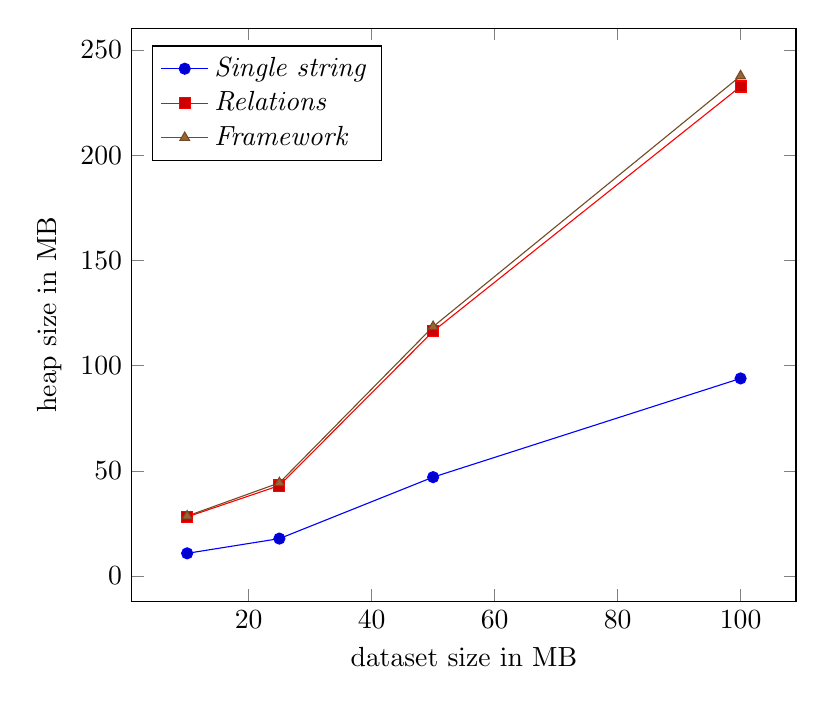
\begin{tikzpicture}
      \begin{axis}[
      scale only axis,
          xlabel=dataset size in MB,
          ylabel=heap size in MB,
          legend pos=north west,
          legend cell align={left},
      ]
        \addplot coordinates {
          (10,10.8) (25,17.8) (50,47.0) (100,93.9)
        };
        \addplot coordinates {
          (10,28.1) (25,43.0) (50,116.3) (100,232.6)
        };
        \addplot+[mark=triangle*] coordinates {
          (10,28.5) (25,44.3) (50,118.5) (100,237.6)
        };
        \legend{\textit{Single string}, \textit{Relations}, \textit{Framework}}
      \end{axis}
    \end{tikzpicture}
    \caption{Used heap size when loading the data into memory using the three different methods.}
    \label{fig:exp:general}
  \end{figure}

  As we can see in \cref{fig:exp:general}, using the full framework with \glspl{dactor} does not introduce much additional memory overhead.
  \Cref{tab:memory_overhead} compares the sizes of the \textit{Relations} and \textit{Framework} tests and lists the \gls{dactor} overhead for the datasets $D_1$ through $D_4$.
  The memory overhead per \gls{dactor} is computed with the following equation:
  \begin{equation}
    \text{Overhead / \gls{dactor}} = \frac{\text{Size \textit{Framework}} - \text{Size \textit{Relations}}}{\text{\# \glspl{dactor}}}
  \end{equation}
  On average, using a \gls{dactor} only needs an additional 533~B more.


\subsection{Discussion}\label{sec:exp:discussion}

  \Cref{tab:memory_overhead} clearly shows that using \glspl{dactor} only introduces a very small memory overhead.
  \Glspl{dactor} have a constant overhead of about 550~B per instance.
  Our experiments show a worst case scenario, where each \gls{dactor} only stores 230~KB on average.

  \begin{table}
    \centering
    \begin{tabular}{crrrr}
      \toprule
      \textbf{Dataset} & \textbf{\# \Glspl{dactor}} & \textbf{Size \textit{Relations}} & \textbf{Size \textit{Framework}} & \textbf{Overhead / \gls{dactor}}\\
      \midrule
      $D_1$ & 829 & 28~788~KB & 29~213~KB & 526~B \\
      $D_2$ & 2~578 & 44~034~KB & 45~392~KB & 539~B \\
      $D_3$ & 4~373 & 119~084~KB & 121~355~KB & 532~B \\
      $D_4$ & 8~618 & 238~169~KB & 242~728~KB & 534~B \\
      % Average overhead = 533B
      \bottomrule
    \end{tabular}
    \caption{Memory overhead of \glspl{dactor}}
    \label{tab:memory_overhead}
  \end{table}
  
  Lets assume, we have a 1~TB database and we chose to store 1~MB per \gls{dactor}.
  This requires the actor database to instantiate about one million \glspl{dactor}.
  Using the average overhead of 550~B per \gls{dactor}, this would yield a relative memory overhead of only $0.05~\%$.
  Doing the same thought experiment with storing 10~MB per \gls{dactor}, results in about 100~000 \glspl{dactor} and reduces the relative memory overhead to $0.005 \%$.

  During execution of the experiments, we noticed that the load times for the \textit{Framework} test were multiple times faster than the other testing scenarios.
  The data loading mechanism in the \textit{Framework} test is highly parallel, because each \gls{dactor} is responsible for loading its data.
  They are triggered by a initial message telling them, where to find the data.


% !TeX root = ../paper.tex
% !TeX encoding = UTF-8
% !TeX spellcheck = en_US

\section{Conclusion}\label{sec:conclusion}

In our research, we study the question how database features can be incorporated into the actor programming model. This initial work presents a proof-of-concept implementation of an actor database framework, which enables developers to declaratively define a data model using \glspl{dactor}.
\Glspl{dactor} model application-domain objects by encapsulating both the object's state and its application logic.
The framework provides a shared, distributed runtime for database functionality and application logic, mitigating the \textit{object-relational impedance mismatch} between data and business logic tier.
%We discuss challenges specific to a database system in a distributed runtime and how the proposed actor database framework solves these challenges.
%In particular, \glspl{dactor} constitute independent units, which allow for flexible partitioning of application data based on application domain logic and concepts.
%The use of the Akka framework enables efficient implementation of partition discovery and failure handling in this distributed setup.
The introduced \gls{functor} concept, which are temporary actors that manage multi-\gls{dactor} queries, provides a transparent computation model and failure handling capabilities.
First experiments with our Akka-based actor database system show that the memory overhead introduced by using actors for data management is low.
%The results show that, due to the constant and low memory footprint of actors, 
Hence, the approach is feasible and pays off especially if large amounts of data need to be stored for highly concurrent data manipulation workloads.
%The research implementation of the framework provides a platform for the integration of traditional database functionalities.
As future work, we aim to develop inter-\gls{dactor} consistency guarantees by extending \gls{functor} with a rollback and, e.g., a \textit{two-phase commit} protocol implementation.
%In addition, further testing of this research implementation's query execution latency and throughput performance remains a topic of interest.
% --------

% bibliography
\printbibliography

\end{document}
